% Dokumentenklasse: 
%   - {article} : fuer Kurzberichte.
% Dokumentenklasseoptionen:
%   - [11pt]    : Schriftgroesse
%   - [a4paper] : Seitenformat DIN A4
%   - [twoside] : zweiseitig bedruckt
%   - [fleqn]   : linksbuendige Ausrichtung der Gleichungen
\documentclass[11pt, a4paper, twoside, fleqn]{article}
% Das Paket inputenc erlaubt die direkte Eingabe von Sonderzeichen wie zum Beispiel deutschen Umlauten,
%  um deren Trennung zu ermoeglichen wird zudem das Paket fontenc mit eingebunden.
\usepackage[utf8]{inputenc}
\usepackage[T1]{fontenc}
\usepackage[greek, english]{babel}
\usepackage{alphabeta}
% Mit fullpage kann die Texthoehe und -breite sowie die Raender festlegen, dass die Seite fast voll ist.
\usepackage{fullpage}
\usepackage{amsmath, amssymb}
\usepackage{multicol}
% With xcolor, pages, the font, frames and fields can be set in the available colors.
\usepackage{xcolor}
\usepackage{tikz}
\usepackage{graphicx}
% Customizable Enumerates/Itemizes
\usepackage{enumitem}
\setlength{\mathindent}{0cm}
\setlength\parindent{0pt}
\setlength{\parskip}{0em}
\renewcommand{\baselinestretch}{1.5}
\title{Άλγεβρα Α' Λυκείου - Τυπολόγιο}
\author{Γιάννης Χριστοδουλάκης}
\date{\selectlanguage{greek}\today}
\graphicspath{{./images/}}
\begin{document}
\maketitle
% The statement ends the current page.
\newpage
% This command causes LaTeX to create a table of contents.
\renewcommand{\contentsname}{Περιεχόμενα}
\tableofcontents
% The statement ends the current page.
\newpage
%%%%%%%%%%%%%%%%%%%%%%%%%%%%%%%%%%%%%%%%%%%%%%%%%%%%%%%%%%%%%%%%%%%%%%
\section{Η έννοια της συνάρτησης}
\begin{flushleft}
\textbf{Συνάρτηση} από ένα σύνολο \(A\) σε ένα σύνολο \(B\) λέγεται μία διαδικασία (κανόνας) με την οποία κάθε στοιχείο του συνόλου \(A\) αντιστοιχίζεται σε ένα ακριβώς στοιχείο του συνόλου \(B\). Το σύνολο \(A\) λέγεται \textbf{πεδίο ορισμού} της \(f\). Όταν δίνεται μόνο ο τύπος μιας συνάρτησης \(f\), τότε θεωρούμε συμβατικά ότι το πεδίο ορισμού \(A\) της \(f\) είναι το ευρύτερο από τα υποσύνολα του $\mathbb{R}$ στα οποία το \(f(x)\) έχει νόημα πραγματικού αριθμού.
\end{flushleft}
\section{Γραφική παράσταση συνάρτησης}
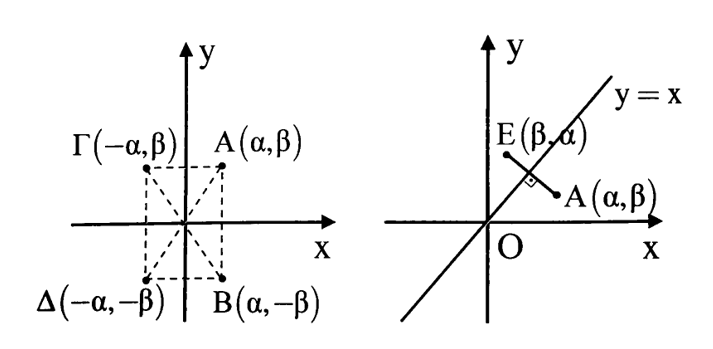
\includegraphics[scale=0.55]{Grafiki_Parastasi}
\begin{flushleft}
Αν Α(α,β) είναι ένα σημείο του καρτεσιανού επιπέδου, τότε το συμμετρικό του:
\end{flushleft}
\begin{itemize}[itemsep=0ex, leftmargin=*]
\item ως προς τον άξονα \(x'x\) είναι το σημείο B(α,-β).
\item ως προς τον άξονα \(y'y\) είναι το σημείο Γ(-α,β).
\item ως προς την αρχή των αξόνων είναι το σημείο Δ(-α,-β).
\item ως προς τη διχοτόμο της 1ης και 3ης γωνίας των αξόνων είναι το σημείο Ε(β,α).
\end{itemize}
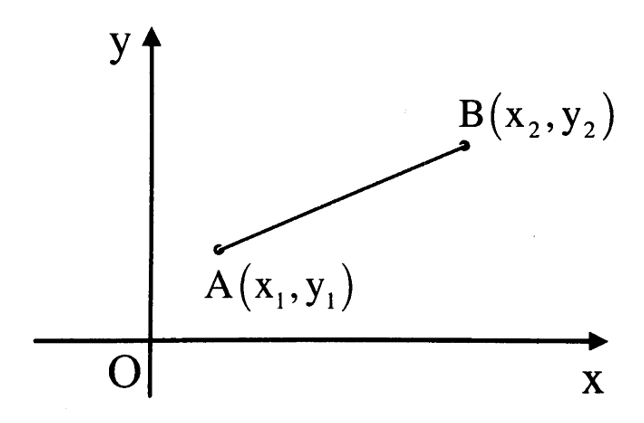
\includegraphics[scale=0.35]{Apostasi}
\begin{flushleft}
Η απόσταση δύο σημείων \(Α(x_{1}, y_{1})\) και \(B(x_{2}, y_{2})\) ενός καρτεσιανού επιπέδου δίνεται από τον τύπο \(AB = \sqrt{(x_{2}-x_{1})^{2} + (y_{2}-y_{1})^{2}}\)
\end{flushleft}
\end{document}